\documentclass[a4paper,10pt]{article}
\usepackage[utf8]{inputenc}
\usepackage{src/preamble}
\usepackage[
	backend=biber,
	maxalphanames=10,
]{biblatex}
\bibliography{bibliography.bib}

\begin{document}

\noindent
\begin{center}
	\textbf{{EFFICIENT SOLUTION FOR MST COMPUTATION ON SPARSE GRAPHS}} \\
\end{center}

\noindent
\textbf{Author: Alessandro Biagiotti} \hfill \textit{Milan university}
\\

\noindent
\textbf{ABSTRACT:}
\\
In this report I will explain my solution for \mstp. In the following sections I will be covering:
The theory behind the problem alongside some solutions~\ref{sec:intro}, the data structure implemented to keep the graph in memory~\ref{sec:graph-structure}, the CPU~\ref{sec:cpu-implementation} and GPU~\ref{sec:gpu-implementation} implementations, the results in terms of speedup and occupancy~\ref{sec:performance-analysis} and finally some conclusions regarding the project and the problem as a whole~\ref{sec:final-thoughts}.

\bigskip

\phantomsection
\makeatletter\def\@currentlabel{\texttt{(I)}}\makeatother\label{sec:intro}
\noindent
\textbf{INTRODUCTION TO THE PROBLEM:}
\\
Given an undirected, weighted and connected graph $\mathcal{G}(V, E)$, computing it's Minimum
Spanning Tree (\mst for short) means finding a minimum weight tree connecting every vertex $v \in V$ in
$\mathcal{G}$.

The Minimum Spanning Tree Problem (\mstp for short) has been studied for years and to this day finds many real world applications, to name a few:
\begin{enumerate}
	\item It's possible to find different \mst-based techniques used to do image segmentation~\cite{maze-generation}~\cite{mst-segmentation-heuristic}.
	\item Finding an \mst allows us to solve the Clustering problem, all we need to do is to compute an \mst and then drop its $k - 1$ most expensive edges~\cite{mst-applications}.
	\item Finding an \mst is an important step of Christofides's algorithm, which is a 2-approximation for the widely known Travelling Salesman Problem (\textsc{Tsp} for short)~\cite{tsp-christofides}.
\end{enumerate}

Many different solutions have been found for the problem in the years, the more basic implementations were Prim's~\cite{prim-algorithm} and Kruskal's~\cite{kruskal-algorithm}.

In the case of Prim's algorithm, given a graph $\mathcal{G} = (V, E)$, let us suppose that the size of the graph $|V|$ is $n$ and the number of edges $|E|$ is $m$, then, based on the implementation, the computational complexity varies:
\begin{itemize}
	\item Na\"ive implementation: $\O(n^2)$
	\item Binary heap and adjacency list: $\O(m\log{n})$
	\item Fibonacci heap and adjacency list: $\O(m + n\log{n})$
\end{itemize}
As will be shown in section~\ref{sec:cpu-implementation} I implemented two different sequential
solvers, the first one using b-heap based Prim's algorithm, and the second one using \brkas algorithm.

Kruskal's algorithm is the alternative to Prim's algorithm and it works in time $\O(m\log{m})$ if
implemented using classical data structures~\cite{clrs}.

\brkas algorithm is a solver for \mstp based on forests, a more verbose version of the algorithm shown in~\cite{boruvka-pseudocode} can be found in~\ref{algo:boruvka-pseudocode}
\begin{algorithm}
	\caption{\brkas algorithm}
	\label{algo:boruvka-pseudocode}
	\begin{algorithmic}[1]
		\REQUIRE An undirected, connected and weighted graph $\mathcal{G}$, an empty set of edges $T$
		\ENSURE An \mst$T$ built on graph $G$
		\WHILE{vertices in $\mathcal{G}$ connected by $T$ are disjoint}
		\STATE start with an empty set of edges $E$
		\FOR{every connected component $\mathcal{C}$}
		\STATE start with an empty set of edges $S$
		\FOR{every vertex $v$ in $\mathcal{C}$}
		\STATE add the cheapest edge going from $v$ to any other component to $S$
		\ENDFOR
		\STATE add the cheapest edge in $S$ to $E$
		\ENDFOR
		\STATE add the set of edges from $E$ to $T$
		\ENDWHILE
		\STATE\RETURN $T$
	\end{algorithmic}
\end{algorithm}

Let us suppose that the size of the graph $|V|$ is $n$ and the number of edges $E$ is $m$, then the computational complexity of the pseudocode shown in~\ref{algo:boruvka-pseudocode} is $\O(m\log{n})$. This algorithm has been later reused in combination with other techniques to compute a solution for the \mstp very efficiently~\cite{boruvka-ackermann}~\cite{karger-klein-tarjan}.

While parallel solutions based on Prim's or Kruskal's algorithm exists like~\cite{prim-parallel}~\cite{filter-kruskal} \brkas solver gained more traction thanks to its inherent parallelizability. Regardless of the implementation the core of the parallel variant can be identified in the following four steps~\cite{boruvka-steps}:
\begin{enumerate}
	\item\label{item:first-step} (\textit{choose lightest}) for every vertex the lightest edge is chosen in parallel.
	\item\label{item:second-step} (\textit{find root}) for every vertex we find the root of the tree to which it belongs\footnote{It's important to keep in mind that vertices are actually supervertices.}.
	\item\label{item:third-step} (\textit{rename vertices}) Since the graph after~\ref{item:fourth-step} undergoes a contraction, the number of vertices decreases, then the roots in the graph need to be renamed.
	\item\label{item:fourth-step} (\textit{graph contraction}) The graph undergoes a contraction, the resulting graph will contain only the roots identified during~\ref{item:second-step} and the edges that connect component $\mathcal{C}_i$ to any other component $\mathcal{C}_j$, any edge contained within a component will be lost.
\end{enumerate}

The specific implementation that I chose to follow is shown in~\cite{generic-he-boruvka} and is summarized by algorithm~\ref{algo:boruvka-parallel}

\begin{algorithm}
	\caption{\brkas algorithm}\label{algo:boruvka-parallel}
	\begin{algorithmic}[1]
		\REQUIRE An undirected, connected and weighted graph $G(V, E)$
		\WHILE{$|V| > 1$}
		\STATE find the minimum edge per vertex (\ref{item:first-step})
		\STATE remove loops
		\STATE initialize the colors
		\WHILE{the coloring hasn't converged}
		\STATE color propagation (\ref{item:second-step})
		\ENDWHILE
		\STATE create new vertex ids (\ref{item:third-step})
		\STATE do graph contraction (\ref{item:fourth-step})
		\ENDWHILE
	\end{algorithmic}
\end{algorithm}

The graph returned in the last step is a single supervertex and the \mst is actually built out of the edges that are pruned in the loop removal process.

\bigskip
\phantomsection
\makeatletter\def\@currentlabel{\texttt{(II)}}\makeatother\label{sec:graph-structure}
\noindent
\textbf{GRAPH STRUCTURE:}
\\
Before discussing the solution I want to briefly introduce the data structure. Normally, when working with graphs, the two data structures that come to mind are:
\begin{itemize}
	\item The \emph{adjacency matrix}, which represents any connection between two vertices, $i,
		j$ in the graph as a $1$ or a $0$ in a matrix in position $(i, j)$\footnote{For simplicity's sale I consider an unweighted graph}. Let's suppose that the $|V|$ is $n$, then the amount of space occupied by a matrix in memory is $\O(n^2)$ while the cost of accessing element $(i, j)$, independently from the values of $i$ and $j$, is just $\O(1)$.
	\item The \emph{adjacency list}, which stores a reference to every neighbour of every vertex. Usually memorized as an array of lists, therefore if $j$ is neighbour for vertex $i$ a reference to $j$ will be placed in the list of neighbours of $i$. Supposing that $|E|$ is $m$, then the cost of keeping such a structure in memory is $O(m + n)$ and the cost of accessing any neighbour for a generic vertex $i$ is going to be $\O(n)$, because in the worst case we could be accessing a graph in which all of the vertices are linked to $i$.
\end{itemize}
The approach I followed for the implementation of the algorithm is, to quote the authors
of~\cite{generic-he-boruvka} "a compromise between adjacency list and adjacency matrix". The \csr
encoding linearizes adjacency lists, to save space, using arrays to keep the adjacency lists in
memory, to save time. The number of additional arrays implemented in \csr varies slightly in the literature~\cite{csr-kelly}~\cite{csr-wheatman}~\cite{generic-he-boruvka}, for my implementation I chose to stray from the 4-vector solution used in~\cite{generic-he-boruvka}, since it would have only complicated the structure of the graph without holding any additional information.
The array structure for my implementation consists of:
\begin{itemize}
	\item A \emph{cumulated degrees} array, it's an array cumulating the degrees of the vertices in the graph, used also to compute the degree of every vertex.
	\item A \emph{neighbours} array, which is a linearization of the graph's adjacency list.
	\item A \emph{weights} array, containing the weight of every edge $(i, j)$ in the graph.
\end{itemize}
An example of the \csr structure is shown in Figure~\ref{tikz:csr-struct}.

\begin{figure}
	\centering
	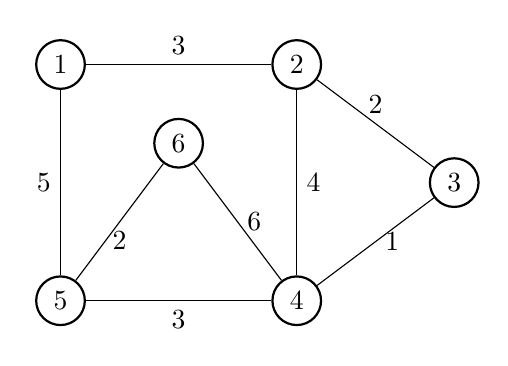
\begin{tikzpicture}

% Define nodes
\node[circle, draw, thick] (1) at (0, 3) {1};
\node[circle, draw, thick] (2) at (3, 3) {2};
\node[circle, draw, thick] (3) at (5, 1.5) {3};
\node[circle, draw, thick] (4) at (3, 0) {4};
\node[circle, draw, thick] (5) at (0, 0) {5};
\node[circle, draw, thick] (6) at (1.5, 2) {6};

% Draw edges with weights
\draw (1) -- (2) node[midway, above] {3};
\draw (1) -- (5) node[midway, left] {5};
\draw (2) -- (3) node[midway, above] {2};
\draw (2) -- (4) node[midway, right] {4};
\draw (3) -- (4) node[midway, right] {1};
\draw (4) -- (5) node[midway, below] {3};
\draw (4) -- (6) node[midway, right] {6};
\draw (5) -- (6) node[midway, below] {2};
\end{tikzpicture}

\begin{tikzpicture}[row 1/.style={nodes={draw}},node distance=6cm]
\matrix(alignedArrays)[matrix of nodes, row sep=0.5cm, nodes={draw, minimum size=6mm}]
{
|[draw=none]| cumulated degrees: & $0$ & $2$ & $5$ & $7$ & $11$ & $14$ & $16$ & |[draw=none]| \\
|[draw=none]| neighbours: & $2$ & $5$ & $1$ & $3$ & $4$ & $2$ & $4$ & $2$ & $3$ & $5$ & $6$ & $1$ & $4$ & $6$ & $4$ & $5$ & |[draw=none]| \\
|[draw=none]| weights: & $3$ & $5$ & $3$ & $2$ & $4$ & $2$ & $1$ & $4$ & $1$ & $3$ & $6$ & $5$ & $3$ & $2$ & $6$ & $2$ & |[draw=none]| \\
};
% Annotate the first row with small numbers
\node[above=1pt of alignedArrays-1-2] {\tiny 1};
\node[above=1pt of alignedArrays-1-3] {\tiny 2};
\node[above=1pt of alignedArrays-1-4] {\tiny 3};
\node[above=1pt of alignedArrays-1-5] {\tiny 4};
\node[above=1pt of alignedArrays-1-6] {\tiny 5};
\node[above=1pt of alignedArrays-1-7] {\tiny 6};

% Annotate the second row with small numbers
\node[above=1pt of alignedArrays-2-2] {\tiny 1};
\node[above=1pt of alignedArrays-2-4] {\tiny 2};
\node[above=1pt of alignedArrays-2-7] {\tiny 3};
\node[above=1pt of alignedArrays-2-9] {\tiny 4};
\node[above=1pt of alignedArrays-2-13] {\tiny 5};
\node[above=1pt of alignedArrays-2-16] {\tiny 6};

% Annotate the third row with small numbers
\node[above=1pt of alignedArrays-3-2] {\tiny 1};
\node[above=1pt of alignedArrays-3-4] {\tiny 2};
\node[above=1pt of alignedArrays-3-7] {\tiny 3};
\node[above=1pt of alignedArrays-3-9] {\tiny 4};
\node[above=1pt of alignedArrays-3-13] {\tiny 5};
\node[above=1pt of alignedArrays-3-16] {\tiny 6};
\end{tikzpicture}
	\caption{An example of a graph's \csr structure}
	\label{tikz:csr-struct}
\end{figure}

\bigskip
\phantomsection
\makeatletter\def\@currentlabel{\texttt{(III)}}\makeatother\label{sec:cpu-implementation}
\noindent
\textbf{CPU IMPLEMENTATION:}
\\
I will not cover at length the CPU implementation since it's quite straightforward, at first I opted
for an extremely na\"ive version of Prim's algorithm, consisting of two \texttt{for} cycles.
Since the algorithm proved to be way too slow I decided to move to a faster solver based on heaps,
which has a time complexity of $\O(m \cdot \log{n})$, as was shown in~\ref{sec:intro}.

I additionally implemented \brkas algortithm which proves to have better performance, as shown in Section \ref{sec:performance-analysis}, when working with sparse graphs.

\bigskip
\phantomsection
\makeatletter\def\@currentlabel{\texttt{(IV)}}\makeatother\label{sec:gpu-implementation}
\noindent
\textbf{GPU IMPLEMENTATION:}
\\
As I alluded to in~\ref{sec:intro} I chose to follow~\cite{generic-he-boruvka} as my primary source. In the paper the researchers propose an higlhly efficient and parallel variant of \brkas solver for the GPU.

Per~\cite{generic-he-boruvka} every part of the solution can be implemented as a distinct kernel
deploying a thread per vertex (such an approach is referred to as \textit{topologic} in the
literature), to better understand every step I took the example graph shown in~\ref{tikz:csr-struct} and I computed the first iteration of the algorithm step-by-step.

Following Algorithm~\ref{algo:boruvka-parallel} one iteration of the outer loop consists of:
\begin{enumerate}
	\item\label{item:choose-lightest} (\textit{choosing the lightest}), as shown in~\ref{tikz:find-cheapest}, this operation picks the lightest outgoing edge in every vertex neighbourhood in parallel. The result is going to be a single reference to the outgoing edge which will be stored in the \texttt{candidates} array.
	
		Weight ties are broken by picking the neighbour with the smallest vertex-id. Considering
		vertex $4$ shown in~\ref{tikz:find-cheapest} the cheapest edge has weight $1$ and
		links $4$ to $3$, therefore in position $4$ inside of the new array we will be
		putting a reference to $3$\footnote{In the actual implementation the offset from the
		beginning of the vertex's neighbourhood is saved}.
	\item\label{item:mirror-removal} (\textit{removing loops}), as shown in~\ref{tikz:loop-removal}, this operation is meant to remove cycles from the graph. Whenever a cycle between vertices $i$ and $j$ is identified only the copy of the edge associated to the vertex with the highest vertex-id is kept, the other is set to the default value of \texttt{UINT\_MAX}.

		Considering vertex $4$ in shown in~\ref{tikz:loop-removal} we see that the candidate
		edge for vertex $3$ leads to $4$, thus a loop has been found, as a result the
		candidate for $3$ is replaced with the default value indicated as $\mathcal{U}$.
	\item\label{item:coloration} (\textit{Initializing and propagating colors}), as shown in~\ref{tikz:coloration}, this operation is meant to identify connected components inside the graph and can be implemented recursively using a kernel as recursion head and a series of \texttt{\_\_device\_\_} function calls to propagate the colors.
	
	The resulting \texttt{colors} array will contain the vertex-id of vertices with undefined candidate value and, for all other vertices, the color value will be computed recursively by using the color of the neighbour pointed by the \texttt{candidates} array.

		If we consider vertex $4$ shown in~\ref{tikz:coloration}, its candidate value is
		pointing to $3$, therefore $4$ will belong to the same component $3$ belongs to,
		since the candidate value for $3$ is $\mathcal{U}$ then it's going to be the root of the
		connected component and its color will be set to its vertex id.
	\item\label{item:vertex-rename} (\textit{Renaming vertices}), as shown in~\ref{tikz:sv-rename}, to rename the vertices a new array is created (in my implementation is \texttt{flag}) that contains a $0$ in every position where the color of the vertex is different from the vertex id and a $1$ otherwise. Afterwards an exclusive scan procedure is comptued on \texttt{flag} to compute the new vertex-ids.

		Since during the previous step the algorithm recursively looks for the root of the
		component we can easily merge the two steps together to have a reduction of the
		kernel launch overhead.
	\item\label{item:graph-contraction} (\textit{Counting, assign and insert new edges}), as shown in the last part of Figure~\ref{tikz:first-iteration} this bigger operation has to be split into three different steps:
	\begin{itemize}
		\item\label{item:count-edges} (\textit{Count edges}), as shown in~\ref{tikz:edge-count}, a simple kernel will be checking every edge in a vertex's neighbourhood, comparing the color of the source with the color of the destination (effectively comparing the connected components they belong to).
		
		If they belong to different connected components the result will be added to the \texttt{newCumDegs} array that is being constructed.
		
			If we consider the neighbourhood for vertex $4$, the first edge leads to
			$2$, which is colored red; since $4$ is colored red as well we do not count
			it as an outgoing edge for the new supervertex (the edge stays within the
			component). $4$ also has an edge leading to vertex $5$ which is colored in
			teal, since its color is not red the edge is reaching another component,
			therefore it is counted as one of the outgoing edges for supervertex $1$.
		\item\label{item:scan-ncd} (\textit{Cumulated degrees computation}), as shown in~\ref{tikz:scan-ncdegs}, the resulting \texttt{newCumDegs}, which contains the outdegrees for every connected component, undergoes a round of scan to finalize the computation of the cumulated degrees vector for the contracted graph.
		\item\label{item:graph-regen} (\textit{Graph contraction}), as shown in~\ref{tikz:graph-contraction}, this step generates the new neighbour and weight array using a logic that is very similar to the one used for the calculation of the new number of outgoing edges.
		
		While edges intra-component are removed, duplicated ones are kept, because it's easier than handling their removal.
	\end{itemize}
\end{enumerate}
Most of the kernels proposed in the solution can be written to use one single thread per vertex and a \texttt{for} loop to cycle the neighbourhood, since there is no dependency between the various vertices~\cite{generic-he-boruvka}, the steps can be computed in parallel for a major efficiency boost. Synchronization is only ever needed inside the \texttt{scan} functions, to make sure that all of the threads have a consistent view of shared memory, atomic operations are required in some instances to offer a solution to race conditions.
\begin{figure}
	    \begin{subfigure}{.7\linewidth}
        \begin{tikzpicture}[row 1/.style={nodes={draw}},node distance=6cm]
            \matrix(alignedArrays)[matrix of nodes, nodes={draw, minimum size=5mm}, row sep=0.25cm]
            {
            |[draw=none]| n: & \color{red}{$2$} & $5$ & $1$ & \color{red}{$3$} & $4$ & $2$ & \color{red}{$4$} & $2$ & \color{red}{$3$} & $5$ & $6$ & $1$ & $4$ & \color{red}{$6$} & $4$ & \color{red}{$5$} & |[draw=none]| \\
            |[draw=none]| w: & \color{red}{$3$} & $5$ & $3$ & \color{red}{$2$} & $4$ & $2$ & \color{red}{$1$} & $4$ & \color{red}{$1$} & $3$ & $6$ & $5$ & $3$ & \color{red}{$2$} & $6$ & \color{red}{$2$} & |[draw=none]| \\
            |[draw=none]| dc: & $2$ & $3$ & $4$ & $3$ & $6$ & $5$ & |[draw=none]| \\
            };

            % Annotate the third row with small numbers
            \node[above=1pt of alignedArrays-1-2] {\tiny 1};
            \node[above=1pt of alignedArrays-1-4] {\tiny 2};
            \node[above=1pt of alignedArrays-1-7] {\tiny 3};
            \node[above=1pt of alignedArrays-1-9] {\tiny 4};
            \node[above=1pt of alignedArrays-1-13] {\tiny 5};
            \node[above=1pt of alignedArrays-1-16] {\tiny 6};
        \end{tikzpicture}
        \caption{\texttt{findCheapest} operation}\label{tikz:find-cheapest}
    \end{subfigure}
    \begin{subfigure}{.3\linewidth}
        \centering
        \begin{tikzpicture}[row 1/.style={nodes={draw}},node distance=6cm]
            \matrix(alignedArrays)[matrix of nodes, nodes={draw, minimum size=5mm, text height=1.5ex, text depth=0.25ex, anchor=base}, row sep=0.25cm]
            {
            |[draw=none]| dc: & $2$ & $3$ & \color{red}{$4$} & \color{red}{$3$} & \color{teal}{$6$} & \color{teal}{$5$} & |[draw=none]| \\
            |[draw=none]| dc: & $2$ & $3$ & $\mathcal{U}$ & $3$ & $\mathcal{U}$ & $5$ & |[draw=none]| \\
            };

            \node[above=1pt of alignedArrays-1-2] {\tiny 1};
            \node[above=1pt of alignedArrays-1-3] {\tiny 2};
            \node[above=1pt of alignedArrays-1-4] {\tiny 3};
            \node[above=1pt of alignedArrays-1-5] {\tiny 4};
            \node[above=1pt of alignedArrays-1-6] {\tiny 5};
            \node[above=1pt of alignedArrays-1-7] {\tiny 6};
        \end{tikzpicture}
        \caption{\texttt{loopRemoval} operation}\label{tikz:loop-removal}
    \end{subfigure}
    \vskip 0.1em
    \begin{subfigure}{.5\linewidth}
        \centering
        \begin{tikzpicture}[row 1/.style={nodes={draw}},node distance=6cm]
            \matrix(alignedArrays)[matrix of nodes, nodes={draw, minimum size=5mm, text height=1.5ex, text depth=0.25ex, anchor=base}, row sep=0.25cm]
            {
            |[draw=none]| dc: & \color{red}{$2$} & \color{red}{$3$} & $\color{red}{\mathcal{U}}$ & \color{red}{$3$} & \color{teal}{$\mathcal{U}$} & \color{teal}{$5$} & |[draw=none]| \\
            |[draw=none]| color: & \color{red}{$3$} & \color{red}{$3$} & \color{red}{$3$} & \color{red}{$3$} & \color{teal}{$5$} & \color{teal}{$5$} & |[draw=none]| \\
            };
            \node[above=1pt of alignedArrays-1-2] {\tiny 1};
            \node[above=1pt of alignedArrays-1-3] {\tiny 2};
            \node[above=1pt of alignedArrays-1-4] {\tiny 3};
            \node[above=1pt of alignedArrays-1-5] {\tiny 4};
            \node[above=1pt of alignedArrays-1-6] {\tiny 5};
            \node[above=1pt of alignedArrays-1-7] {\tiny 6};
        \end{tikzpicture}
        \caption{\texttt{coloration} operation}\label{tikz:coloration}
    \end{subfigure}
    \begin{subfigure}{.5\linewidth}
        \centering
        \begin{tikzpicture}[row 1/.style={nodes={draw}},node distance=6cm]
            \matrix(alignedArrays)[matrix of nodes, nodes={draw, minimum size=5mm, text height=1.5ex, text depth=0.25ex, anchor=base}, row sep=0.25cm]
            {
            |[draw=none]| color: & \color{red}{$3$} & \color{red}{$3$} & \color{red}{$3$} & \color{red}{$3$} & \color{teal}{$5$} & \color{teal}{$5$} & |[draw=none]| \\
            |[draw=none]| flag: & $0$ & $0$ & $1$ & $0$ & $1$ & $0$ & |[draw=none]| \\
            |[draw=none]| flag: & $0$ & $0$ & $0$ & $1$ & $1$ & $2$ & |[draw=none]| \\
            };
            \node[above=1pt of alignedArrays-1-2] {\tiny 1};
            \node[above=1pt of alignedArrays-1-3] {\tiny 2};
            \node[above=1pt of alignedArrays-1-4] {\tiny 3};
            \node[above=1pt of alignedArrays-1-5] {\tiny 4};
            \node[above=1pt of alignedArrays-1-6] {\tiny 5};
            \node[above=1pt of alignedArrays-1-7] {\tiny 6};
        \end{tikzpicture}
        \caption{\texttt{svRename} operation}\label{tikz:sv-rename}
    \end{subfigure}
    \vskip 0.1em
    \begin{subfigure}{.7\linewidth}
        \begin{tikzpicture}[row 1/.style={nodes={draw}},node distance=6cm]
            \matrix(alignedArrays)[matrix of nodes, nodes={draw, minimum size=5mm, text height=1.5ex, text depth=0.25ex, anchor=base}, row sep=0.35cm]
            {
            |[draw=none]| color: & \color{red}{$3$} & \color{red}{$3$} & \color{red}{$3$} & \color{red}{$3$} & \color{teal}{$5$} & \color{teal}{$5$} & |[draw=none]| \\
            |[draw=none]| flag: & $0$ & $0$ & $0$ & $1$ & $1$ & $2$ & |[draw=none]| \\
            |[draw=none]| n: & \color{red}{$2$} & \color{teal}{$5$} & \color{red}{$1$} & \color{red}{$3$} & \color{red}{$4$} & \color{red}{$2$} & \color{red}{$4$} & \color{red}{$2$} & \color{red}{$3$} & \color{teal}{$5$} & \color{teal}{$6$} & \color{red}{$1$} & \color{red}{$4$} & \color{teal}{$6$} & \color{red}{$4$} & \color{teal}{$5$} & |[draw=none]| \\
            |[draw=none]| ncDegs: & $3$ & $3$ & $0$ & |[draw=none]| \\
            };
            \node[above=1pt of alignedArrays-1-2] {\tiny 1};
            \node[above=1pt of alignedArrays-1-3] {\tiny 2};
            \node[above=1pt of alignedArrays-1-4] {\tiny 3};
            \node[above=1pt of alignedArrays-1-5] {\tiny 4};
            \node[above=1pt of alignedArrays-1-6] {\tiny 5};
            \node[above=1pt of alignedArrays-1-7] {\tiny 6};

            % Annotate the third row with small numbers
            \node[above=1pt of alignedArrays-3-2] {\tiny 1};
            \node[above=1pt of alignedArrays-3-4] {\tiny 2};
            \node[above=1pt of alignedArrays-3-7] {\tiny 3};
            \node[above=1pt of alignedArrays-3-9] {\tiny 4};
            \node[above=1pt of alignedArrays-3-13] {\tiny 5};
            \node[above=1pt of alignedArrays-3-16] {\tiny 6};
        \end{tikzpicture}
        \caption{\texttt{edgeCount} operation}\label{tikz:edge-count}
    \end{subfigure}
    \begin{subfigure}{.3\linewidth}
        \centering
        \begin{tikzpicture}[row 1/.style={nodes={draw}},node distance=6cm]
            \matrix(alignedArrays)[matrix of nodes, nodes={draw, minimum size=5mm, text height=1.5ex, text depth=0.25ex, anchor=base}, row sep=0.25cm]
            {
            |[draw=none]| ncDegs: & $3$ & $3$ & $0$ & |[draw=none]| \\
            |[draw=none]| ncDegs: & $0$ & $3$ & $6$ & |[draw=none]| \\
            };
            \node[above=1pt of alignedArrays-1-3] {\tiny 1};
            \node[above=1pt of alignedArrays-1-4] {\tiny 2};
        \end{tikzpicture}
        \caption{\texttt{scan} operation on ncDegs}\label{tikz:scan-ncdegs}
    \end{subfigure}
    \vskip 0.1em
    \begin{subfigure}{\linewidth}
        \centering
        \begin{tikzpicture}[row 1/.style={nodes={draw}},node distance=6cm]
            \matrix(alignedArrays)[matrix of nodes, nodes={draw, minimum size=5mm}, row sep=0.25cm]
            {
            |[draw=none]| ncDegs: & $0$ & $3$ & $6$ & |[draw=none]| \\
            |[draw=none]| n: & \color{red}{$2$} & \color{teal}{$5$} & \color{red}{$1$} & \color{red}{$3$} & \color{red}{$4$} & \color{red}{$2$} & \color{red}{$4$} & \color{red}{$2$} & \color{red}{$3$} & \color{teal}{$5$} & \color{teal}{$6$} & \color{red}{$1$} & \color{red}{$4$} & \color{teal}{$6$} & \color{red}{$4$} & \color{teal}{$5$} & |[draw=none]| \\
            |[draw=none]| w: & $3$ & $5$ & $3$ & $2$ & $4$ & $2$ & $1$ & $4$ & $1$ & $3$ & $6$ & $5$ & $3$ & $2$ & $6$ & $2$ & |[draw=none]| \\
            |[draw=none]| nn: & $5$ & $5$ & $6$ & $1$ & $4$ & $4$ & |[draw=none]| \\
            |[draw=none]| nw: & $5$ & $3$ & $6$ & $5$ & $3$ & $6$ & |[draw=none]| \\
            };
            \node[above=1pt of alignedArrays-1-3] {\tiny 1};
            \node[above=1pt of alignedArrays-1-4] {\tiny 2};
            \node[above=1pt of alignedArrays-4-2] {\tiny 1};
            \node[above=1pt of alignedArrays-4-5] {\tiny 2};
            \node[above=1pt of alignedArrays-5-2] {\tiny 1};
            \node[above=1pt of alignedArrays-5-5] {\tiny 2};
        \end{tikzpicture}
        \caption{\texttt{scan} operation on ncDegs}\label{tikz:graph-contraction}
    \end{subfigure}
	\caption{Example of the first iteration}\label{tikz:first-iteration}
\end{figure}
In the following section I will be comparing two very similar approaches, GPU-u, which follows
closely the implementation guidelines of the original paper, and GPU-e, which is more experimental.
GPU-e differs essentially in how it computes the new cumulated degrees vector and the graph
contraction; instead of using a topological approach for both kernels I use one thread per edge and
then proceed to do a binary search for each edge to find the source of the edge. While this approach
is not scalable by definition due to the extreme requirements it might need to satisfy it bears the
germ of an idea that might prove interesting if more effort was to be put into it, more on this in
section~\ref{sec:final-thoughts}.

\bigskip
\phantomsection
\makeatletter\def\@currentlabel{\texttt{(III)}}\makeatother\label{sec:performance-analysis}
\noindent
\textbf{PERFORMANCE ANALYSIS:}
\\
Development and performance analysis have been carried out using the Google Colab hosting service\footnote{\url{https://colab.research.google.com/}}, the machine specs, gathered through tools like \texttt{/proc/cpuinfo} and \texttt{/proc/meminfo}, alongside \texttt{nvidia-smi} and the official documentation~\cite{t4-info}~\cite{t4-product-brief}, are listed in~\ref{tbl:system}
\begin{center}
	\begin{longtable}{|c|c|c|}
		\caption{System information}\label{tbl:system}
		\\\hline\textbf{} & \textbf{CPU} & \textbf{GPU} \\\hline\hline
		\endfirsthead\hline\endlastfoot

		\textbf{Manufacturer}               & Intel                                                                                                               & NVIDIA                                                              \\\hline

		\textbf{Model}                      & Intel Xeon (V\footnote{V stands for virtualized, can't find the actual CPU model that is being mounted in servers}) & T4                                                                  \\\hline
		\textbf{Launch Date}                & N.A.                                                                                                                & Oct 2018                                                            \\\hline
		\textbf{\#Cores}                    & $2$ vcores                                                                                                          & $\num{2560}$ C\footnote{CUDA cores}, $320$ T\footnote{Tensor cores} \\\hline
		\textbf{Clock Speed (GHz)}          & $\num{2.20}$ GHz                                                                                                    & Base: $0.585$ MHz, Boost: $1.59$ GHz                                \\\hline
		\textbf{Memory / Cache}             & L3 Cache: $56$ MB                                                                                                   & VRAM: $16$ GB GDDR6                                                 \\\hline
		\textbf{Memory Bandwidth}           & N.A.                                                                                                                & 300 GB/s                                                            \\\hline
		\textbf{TDP (Thermal Design Power)} & N.A.                                                                                                                & $70$ W                                                              \\\hline
		\textbf{Architecture}               & N.A.                                                                                                                & Turing
	\end{longtable}
\end{center}
All of the benchmarks conducted are part of the tests provided for DIMACS\footnote{DIscrete
MAthematics \& theoretical Computer Science center
(\url{https://www.diag.uniroma1.it/challenge9/download.shtml})} 9th challenge, the benchmark
instances are listed in table~\ref{tbl:benchmarks} and the results for the original paper have been
plotted alongside mine, for reference, in~\ref{fig:results}.
\begin{longtable}{|c|c|c|}
	\caption{Benchmark dimensions}\label{tbl:benchmarks}
	\\\hline\textbf{Benchmark} & \textbf{Node size} & \textbf{Edge size} \\\hline\hline
	\endfirsthead\hline\endlastfoot

	\textit{New York}                & $\num{264346}$   & $\num{733846}$  \\\hline
	\textit{San Francisco, bay area} & $\num{321270}$   & $\num{800172}$  \\\hline
	\textit{Colorado}                & $\num{435666}$   & $\num{1057066}$ \\\hline
	\textit{Florida}                 & $\num{1070376}$  & $\num{2712798}$ \\\hline
	\textit{California and Nevada}   & $\num{1890815}$ & $\num{4657742}$ \\\hline
	\textit{Great Lakes}             & $\num{2758119}$  & $\num{6885658}$ \\\hline
	\textit{Eastern USA}             & $\num{3598623}$  & $\num{8778114}$
\end{longtable}
The testing results plotted in~\ref{fig:results} were obtained by running every benchmark $5$ times for both GPU approaches, average and standard deviation for the timings were then computed and plotted.
\begin{figure}
	\centering
	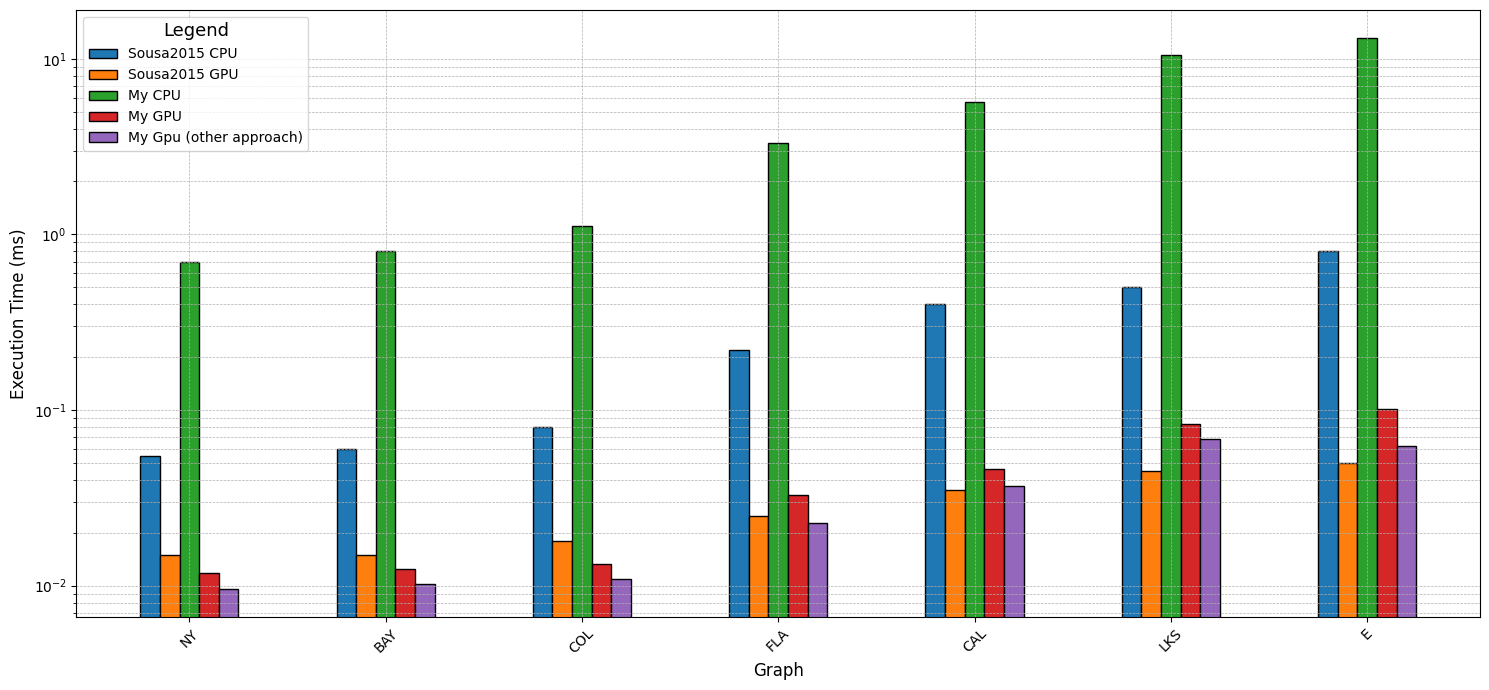
\includegraphics[scale=0.4]{fig/benchmarks.png}
	\caption{Performance metrics for the various platforms compared with the results in \cite{generic-he-boruvka}}
	\label{fig:results}
\end{figure}
Considering the various CPU implementations plotted in Figure~\ref{fig:results} speedup for GPU-e, with respect to \brka implementation, ranges between $\sim42\times$ and $\sim92\times$, while the speedup for GPU-u ranges between $\sim33\times$ and $\sim83\times$. Considering Prim's implementation the speedup for GPU-e ranges between $\sim66\times$ and $\sim150\times$, while the speedup for GPU-u ranges between $\sim52\times$ and $\sim136\times$.

Comparing my GPU implementations with the CPU approaches proposed in\cite{generic-he-boruvka}, based
on OpenMP, we can see that both of my solutions consistently beat the single-threaded version (seen
in Figure~\ref{fig:results}) with an estimated speedup between $\sim5\times$ and $\sim10\times$
while the speedup for the multithreaded implementation is closer to $1$ (which can only be found in
the source material)\footnote{All comparisons the original paper have to be taken with a grain of
salt, the algorithm was not rerun on my machine, I decided to include the results in the analysis
just for reference but they weren't used as actual benchmark for my solution.}.

\medskip
The \emph{occupancy} metric for a kernel $\mathcal{K}$ on a GPU is defined as the ratio of active
warps on an SM to the maximum number of active warps supported by the SM~\cite{def-occupancy}. To
test for it, Nvidia provides the tool Nsight Compute (\texttt{ncu}). The results have been plotted
in figure~\ref{fig:occupancy}, as we can see the general occupancy is inversely proportional to the
number of iterations, that was to be expected because I followed a topologic approach, which means
that the number of threads used by each kernel is going to be just as many as it's required to
occupy every single thread with the computation for one vertex (while having some extras). Since I
decided to have threads arranged in a static single-dimension block of 1024 the result is that the
number of active threads at the end of the algorithm (in the last couple of iterations) is really
low, compared to the total threads available.
\begin{figure}[!h]
	\centering
	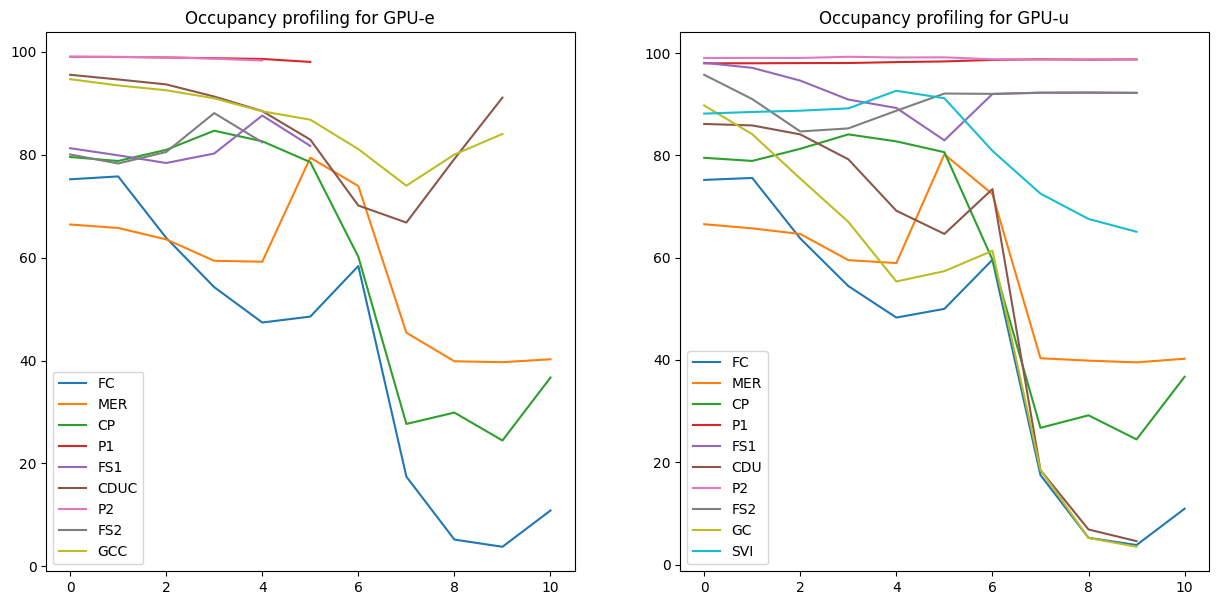
\includegraphics[scale=0.5]{fig/occupancy.png}
	\caption{Occupancy measurements for the two different approaches}
	\label{fig:occupancy}
\end{figure}

\bigskip
\phantomsection
\makeatletter\def\@currentlabel{\texttt{(IV)}}\makeatother\label{sec:final-thoughts}
\noindent
\textbf{CONCLUSIONS:}
\\
\mstp will never stop to amaze due to how much can be done with the solution to a relatively simple problem. As I explained in~\ref{sec:intro} \mstp solvers have been used and are being used extensively to solve a wide gamma of larger problems, therefore there is no "being too fast".

In the previous sections I explained how I got to the solution following somebody else's footsteps but, as always, more work can be done.

Although the original paper was published under the title "A generic and highly efficient parallel variant of \brkas algorithm" it's immediately clear by taking a look at what kind of tests have been done on the solver (all similar to~\ref{tbl:benchmarks}) that the solution is not as "generic" as the authors would like it to be, and it's highly likely it will keep on performing on graphs with limited density.

As shown in Section~\ref{sec:performance-analysis} the results obtained by trying a different
approach yielded mixed results on average, therefore it's not entirely clear whether an approach
entirely based on visiting edges (which would be based on the use of segmented scan) instead of vertices would be beneficial, and lead to better results, or detrimental, because of the heavy use of atomic operations and synchronization.

It would be interesting, to keep experimenting and finding different ways of computing \mst in
parallel like~\cite{mst-bipartite} especially targetting graphs with higher densities.

\clearpage

\printbibliography

\end{document}
